% TODO checklist:
% [x] Inspected: src/resilience/llm_fallback.py (circuit breaker, cost tracking, fallback orchestrator)
% [x] Inspected: src/services/orchestrator.py (LLM client management, provider selection)
% [x] Inspected: src/adapters/llm.py (LLM client implementation)
% [x] Inspected: db/postgres_control/models/providers.py (provider model)
% [x] Inspected: db/postgres_control/models/model_instances.py (model instance model)
% [x] Inspected: Q&A.md (Questions 23-28 on LLM providers, resilience, cost tracking)
% [x] Inspected: README.md (multi-provider LLM support overview)

\section{LLM Provider Management}
\label{sec:llm-providers}

Large Language Model (LLM) provider management is a critical subsystem of the orchestration engine, responsible for selecting, invoking, and monitoring the language models that power agent reasoning and generation. This section examines the provider registry architecture, model resolution strategies, and the resilience framework that ensures reliable operation across diverse deployment environments.

\subsection{Provider Registry Architecture}

The platform implements a database-backed provider registry that enables dynamic management of LLM providers without code changes or redeployment.

\subsubsection{Provider Model}

Providers are registered as entities in the PostgreSQL control plane:

\begin{lstlisting}[language=Python, caption={Provider model structure}, label=lst:provider-model]
class Provider(Base):
    """LLM provider configuration."""
    __tablename__ = "providers"
    
    id: UUID                    # Unique identifier
    tenant_id: str              # Tenant scope
    name: str                   # Display name (e.g., "OpenAI GPT-4")
    provider_type: str          # openai | ollama | azure | anthropic
    base_url: str               # API endpoint
    api_key_ref: str | None     # Reference to secret store
    is_enabled: bool            # Active/inactive status
    is_default: bool            # Default provider for tenant
    priority: int               # Fallback priority (lower = higher priority)
    max_tokens_per_request: int # Token limit
    timeout_seconds: float      # Request timeout
    
    # Circuit breaker settings
    failure_threshold: int      # Failures before opening
    recovery_timeout: int       # Seconds before half-open
    success_threshold: int      # Successes to close
    
    # Cost tracking
    cost_per_1k_input: float    # USD per 1K input tokens
    cost_per_1k_output: float   # USD per 1K output tokens
    max_cost_per_hour: float    # Hourly cost cap
    
    created_at: datetime
    updated_at: datetime
\end{lstlisting}

\subsubsection{Model Instance Model}

Model instances represent specific models available through providers:

\begin{lstlisting}[language=Python, caption={Model instance structure}, label=lst:model-instance]
class ModelInstance(Base):
    """Specific model configuration."""
    __tablename__ = "model_instances"
    
    id: UUID                    # Unique identifier
    provider_id: UUID           # Parent provider
    tenant_id: str              # Tenant scope
    model_id: str               # Model identifier (e.g., "gpt-4-turbo")
    display_name: str           # Human-readable name
    context_length: int         # Maximum context window
    is_enabled: bool            # Active/inactive status
    is_default: bool            # Default model for tenant
    
    # Capabilities
    supports_functions: bool    # Function calling support
    supports_vision: bool       # Vision/multimodal support
    supports_streaming: bool    # Response streaming
    
    # Usage tracking
    total_requests: int         # Lifetime request count
    total_input_tokens: int     # Lifetime input tokens
    total_output_tokens: int    # Lifetime output tokens
    total_cost: float           # Lifetime cost
    
    created_at: datetime
    updated_at: datetime
\end{lstlisting}

\subsubsection{Default Model Resolver (DMR)}

The Default Model Resolver (DMR) determines which model to use for a given request:

\begin{lstlisting}[language=Python, caption={Default model resolution logic}, label=lst:dmr-resolution]
def resolve_model(
    tenant_id: str,
    requested_model: str | None = None,
    intent: str | None = None,
    capabilities: list[str] | None = None,
) -> ModelInstance:
    """Resolve the model to use for a request."""
    
    # 1. If model explicitly requested, use it
    if requested_model:
        model = get_model_by_name(tenant_id, requested_model)
        if model and model.is_enabled:
            return model
    
    # 2. Check tenant-level default
    tenant = get_tenant(tenant_id)
    if tenant.default_model_id:
        model = get_model(tenant.default_model_id)
        if model and model.is_enabled:
            return model
    
    # 3. Find first enabled model meeting capability requirements
    models = list_models(tenant_id, enabled_only=True)
    for model in sorted(models, key=lambda m: m.provider.priority):
        if meets_capabilities(model, capabilities):
            return model
    
    raise NoAvailableModelError("No suitable model found")
\end{lstlisting}

The resolution priority is:
\begin{enumerate}
    \item Explicitly requested model (from API parameter)
    \item Tenant-configured default model
    \item First available model by provider priority meeting capability requirements
\end{enumerate}

\subsection{Resilience Framework}
\label{subsec:resilience-framework}

The resilience framework, implemented in \texttt{src/resilience/llm\_fallback.py}, provides fault-tolerant LLM calling with automatic failover, circuit breakers, and cost governance.

\subsubsection{LLMFallbackOrchestrator}

The \texttt{LLMFallbackOrchestrator} class coordinates resilient LLM calls:

\begin{lstlisting}[language=Python, caption={LLMFallbackOrchestrator structure}, label=lst:fallback-orchestrator]
class LLMFallbackOrchestrator:
    """Orchestrates LLM calls with fallback, circuit breaker, and cost tracking."""
    
    def __init__(
        self,
        providers: dict[str, LLMProvider],
        configs: list[ProviderConfig],
    ):
        self.providers = providers
        self.configs = {c.name: c for c in sorted(configs, key=lambda x: x.priority)}
        
        # Circuit breakers per provider
        self.circuit_breakers = {
            name: CircuitBreaker(
                provider_name=name,
                failure_threshold=config.failure_threshold,
                recovery_timeout=config.recovery_timeout,
                success_threshold=config.success_threshold,
            )
            for name, config in self.configs.items()
        }
        
        # Cost trackers per provider
        self.cost_trackers = {
            name: CostTracker(max_cost_per_hour=config.max_cost_per_hour)
            for name, config in self.configs.items()
        }
        
        # Statistics
        self.stats = {
            "total_calls": 0,
            "successful_calls": 0,
            "failed_calls": 0,
            "fallback_calls": 0,
            "cost_limited_calls": 0,
            "circuit_breaker_blocks": 0,
        }
\end{lstlisting}

\subsubsection{Call Flow with Resilience Checks}

Each LLM call proceeds through multiple resilience checks:

\begin{lstlisting}[language=Python, caption={Resilient LLM call flow}, label=lst:resilient-call]
async def call(
    self,
    prompt: str,
    max_tokens: int = 1000,
    temperature: float = 0.7,
    **kwargs,
) -> dict[str, Any]:
    """Call LLM with automatic fallback."""
    
    errors = []
    attempted_providers = []
    
    # Try providers in priority order
    for provider_name, config in self.configs.items():
        if not config.enabled:
            continue
        
        attempted_providers.append(provider_name)
        
        # Check 1: Circuit breaker
        circuit = self.circuit_breakers[provider_name]
        if not circuit.can_attempt():
            errors.append(f"{provider_name}: Circuit breaker {circuit.state}")
            continue
        
        # Check 2: Cost cap
        cost_tracker = self.cost_trackers[provider_name]
        if not cost_tracker.can_afford(max_tokens, provider_name):
            errors.append(f"{provider_name}: Cost cap exceeded")
            continue
        
        # Check 3: Token limit
        if max_tokens > config.max_tokens_per_request:
            errors.append(f"{provider_name}: Token limit exceeded")
            continue
        
        # Attempt call
        try:
            result = await asyncio.wait_for(
                self.providers[provider_name].call(prompt, max_tokens, temperature),
                timeout=config.timeout_seconds,
            )
            
            circuit.record_success()
            cost_tracker.record_usage(provider_name, result["input_tokens"], result["output_tokens"])
            
            return {**result, "provider": provider_name, "fallback_used": len(attempted_providers) > 1}
            
        except Exception as e:
            circuit.record_failure()
            errors.append(f"{provider_name}: {e}")
            continue
    
    raise Exception(f"All providers failed: {errors}")
\end{lstlisting}

\subsection{Budgeting and Cost Governance}
\label{subsec:budgeting}

The platform implements comprehensive cost tracking and governance to prevent budget overruns and enable chargeback accounting.

\subsubsection{Cost Calculation}

Token-based cost calculation uses provider-specific pricing:

\begin{lstlisting}[language=Python, caption={Cost calculation}, label=lst:cost-calc]
@dataclass
class CostTracker:
    """Track provider costs and enforce caps."""
    
    max_cost_per_hour: float
    window_size_seconds: int = 3600  # 1 hour sliding window
    
    # Cost per 1K tokens by provider
    PROVIDER_COSTS = {
        "openai-gpt4": {"input": 0.03, "output": 0.06},
        "openai-gpt35": {"input": 0.001, "output": 0.002},
        "anthropic-claude": {"input": 0.008, "output": 0.024},
        "azure-openai": {"input": 0.03, "output": 0.06},
        "ollama": {"input": 0.0, "output": 0.0},  # Self-hosted is free
    }
    
    def record_usage(self, provider: str, input_tokens: int, output_tokens: int) -> float:
        """Record token usage and return cost."""
        pricing = self.PROVIDER_COSTS.get(provider, {"input": 0.01, "output": 0.02})
        
        cost = (input_tokens / 1000.0 * pricing["input"]) + \
               (output_tokens / 1000.0 * pricing["output"])
        
        self.costs.append({
            "timestamp": time.time(),
            "provider": provider,
            "input_tokens": input_tokens,
            "output_tokens": output_tokens,
            "cost": cost,
        })
        
        self._cleanup_old_costs()  # Remove entries outside window
        return cost
\end{lstlisting}

\subsubsection{Budget Enforcement}

Pre-call budget checks prevent exceeding configured limits:

\begin{lstlisting}[language=Python, caption={Budget enforcement}, label=lst:budget-enforcement]
def can_afford(self, estimated_tokens: int, provider: str) -> bool:
    """Check if request is within cost cap."""
    current_cost = self.get_current_cost()
    
    # Estimate cost for this request (assume 50/50 input/output)
    pricing = self.PROVIDER_COSTS.get(provider, {"input": 0.01, "output": 0.02})
    estimated_cost = (estimated_tokens / 2000.0 * pricing["input"]) + \
                     (estimated_tokens / 2000.0 * pricing["output"])
    
    return (current_cost + estimated_cost) <= self.max_cost_per_hour

def get_stats(self) -> dict[str, Any]:
    """Get cost statistics."""
    self._cleanup_old_costs()
    total_cost = sum(c["cost"] for c in self.costs)
    
    return {
        "current_cost": total_cost,
        "max_cost_per_hour": self.max_cost_per_hour,
        "remaining_budget": max(0, self.max_cost_per_hour - total_cost),
        "utilization_pct": min(100, (total_cost / self.max_cost_per_hour) * 100),
        "total_input_tokens": sum(c["input_tokens"] for c in self.costs),
        "total_output_tokens": sum(c["output_tokens"] for c in self.costs),
        "request_count": len(self.costs),
    }
\end{lstlisting}

\subsubsection{Cost Aggregation Levels}

Costs are tracked at multiple granularities:

\begin{table}[htbp]
\centering
\caption{Cost tracking granularities}
\label{tab:cost-granularities}
\begin{tabular}{ll}
\hline
\textbf{Level} & \textbf{Description} \\
\hline
Per-Request & Individual LLM call cost \\
Per-Session & Aggregated across session runs \\
Per-Run & Total cost of an agent run \\
Per-Tenant & Tenant-level aggregation for billing \\
Per-Provider & Provider utilization analysis \\
\hline
\end{tabular}
\end{table}

\subsection{Circuit Breaker Implementation}
\label{subsubsec:circuit-breaker}

The circuit breaker pattern prevents cascade failures when LLM providers experience issues.

\subsubsection{State Machine}

The circuit breaker implements a three-state machine:

\begin{figure}[htbp]
\centering
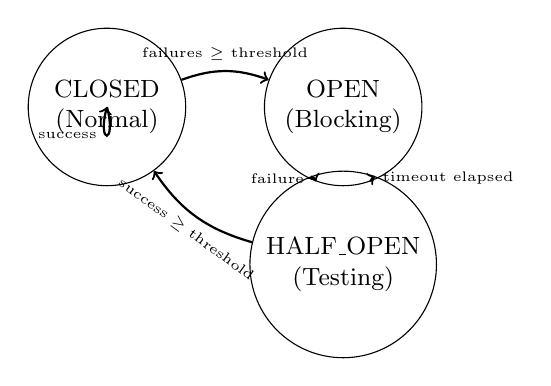
\begin{tikzpicture}[
    node distance=3cm,
    state/.style={circle, draw, minimum size=2cm, align=center, font=\small},
    arrow/.style={->, thick, bend left=20}
]
    % States
    \node[state] (closed) {CLOSED\\(Normal)};
    \node[state, right of=closed] (open) {OPEN\\(Blocking)};
    \node[state, below of=open, yshift=1cm] (half) {HALF\_OPEN\\(Testing)};
    
    % Transitions
    \draw[arrow] (closed) to node[above, font=\tiny] {failures $\geq$ threshold} (open);
    \draw[arrow] (open) to node[right, font=\tiny] {timeout elapsed} (half);
    \draw[arrow] (half) to node[below, font=\tiny, sloped] {success $\geq$ threshold} (closed);
    \draw[arrow] (half) to node[left, font=\tiny] {failure} (open);
    \draw[arrow, loop left] (closed) to node[left, font=\tiny] {success} (closed);
\end{tikzpicture}
\caption{Circuit breaker state machine}
\label{fig:circuit-breaker}
\end{figure}

\begin{description}
    \item[CLOSED] Normal operation. Requests pass through to the provider. Successes reset failure count; failures increment it. When failures reach the threshold, the circuit opens.
    
    \item[OPEN] Blocking mode. Requests fail immediately without attempting the provider. After the recovery timeout elapses, the circuit transitions to half-open.
    
    \item[HALF\_OPEN] Recovery testing. A limited number of requests are allowed through. If they succeed, the circuit closes. If any fail, the circuit reopens.
\end{description}

\subsubsection{Implementation}

\begin{lstlisting}[language=Python, caption={CircuitBreaker implementation}, label=lst:circuit-breaker]
@dataclass
class CircuitBreaker:
    """Circuit breaker for a single provider."""
    
    provider_name: str
    failure_threshold: int = 5      # Failures before opening
    recovery_timeout: int = 60      # Seconds before half-open
    success_threshold: int = 2      # Successes to close
    
    state: CircuitState = CircuitState.CLOSED
    failure_count: int = 0
    success_count: int = 0
    last_failure_time: float | None = None
    opened_at: float | None = None
    
    def record_success(self) -> None:
        """Record successful request."""
        if self.state == CircuitState.HALF_OPEN:
            self.success_count += 1
            if self.success_count >= self.success_threshold:
                self._close()
        elif self.state == CircuitState.CLOSED:
            self.failure_count = 0  # Reset on success
    
    def record_failure(self) -> None:
        """Record failed request."""
        self.last_failure_time = time.time()
        
        if self.state == CircuitState.HALF_OPEN:
            self._open()  # Failed during recovery
        elif self.state == CircuitState.CLOSED:
            self.failure_count += 1
            if self.failure_count >= self.failure_threshold:
                self._open()
    
    def can_attempt(self) -> bool:
        """Check if request can be attempted."""
        if self.state == CircuitState.CLOSED:
            return True
        
        if self.state == CircuitState.OPEN:
            if self.opened_at and time.time() - self.opened_at >= self.recovery_timeout:
                self._half_open()
                return True
            return False
        
        return True  # HALF_OPEN allows attempts
\end{lstlisting}

\subsubsection{Configuration Parameters}

Circuit breaker behavior is configurable per provider:

\begin{table}[htbp]
\centering
\caption{Circuit breaker configuration parameters}
\label{tab:circuit-params}
\begin{tabular}{llr}
\hline
\textbf{Parameter} & \textbf{Description} & \textbf{Default} \\
\hline
\texttt{failure\_threshold} & Failures before opening & 5 \\
\texttt{recovery\_timeout} & Seconds before half-open & 60 \\
\texttt{success\_threshold} & Successes to close & 2 \\
\hline
\end{tabular}
\end{table}

\subsubsection{Failure Detection}

The circuit breaker detects failures from:
\begin{itemize}
    \item HTTP 5xx responses (server errors)
    \item Connection timeouts
    \item Rate limit responses (HTTP 429)
    \item Configurable exception types
\end{itemize}

\subsection{Cost Tracking}
\label{subsubsec:cost-tracking}

Cost tracking provides visibility into LLM usage for budgeting and optimization.

\subsubsection{Per-Model Pricing}

Pricing is configured per model, enabling accurate cost calculation across heterogeneous deployments:

\begin{lstlisting}[language=Python, caption={Model pricing configuration}, label=lst:model-pricing]
MODEL_PRICING = {
    "gpt-4-turbo": {
        "input_per_1k": 0.01,
        "output_per_1k": 0.03,
        "context_length": 128000,
    },
    "gpt-3.5-turbo": {
        "input_per_1k": 0.0005,
        "output_per_1k": 0.0015,
        "context_length": 16385,
    },
    "phi3-mini-instruct": {
        "input_per_1k": 0.0,  # Self-hosted
        "output_per_1k": 0.0,
        "context_length": 4096,
    },
}
\end{lstlisting}

\subsubsection{Sliding Window Tracking}

Cost tracking uses a sliding window for budget enforcement:

\begin{lstlisting}[language=Python, caption={Sliding window cost tracking}, label=lst:sliding-window]
def _cleanup_old_costs(self) -> None:
    """Remove cost entries outside window."""
    cutoff = time.time() - self.window_size_seconds
    self.costs = [c for c in self.costs if c["timestamp"] >= cutoff]

def get_current_cost(self) -> float:
    """Get total cost in current window."""
    self._cleanup_old_costs()
    return sum(c["cost"] for c in self.costs)
\end{lstlisting}

\subsubsection{Self-Hosted Models}

For self-hosted models (e.g., Ollama), cost tracking can be disabled or configured with nominal values:

\begin{itemize}
    \item Zero cost for self-hosted inference
    \item Optional resource utilization tracking (GPU time, memory)
    \item Compute-based cost attribution for infrastructure accounting
\end{itemize}

\subsection{Provider Fallback Strategy}
\label{subsubsec:fallback-strategy}

The fallback strategy ensures high availability by routing to backup providers when the primary is unavailable.

\subsubsection{Fallback Chain}

Providers are ordered by priority, forming a fallback chain:

\begin{enumerate}
    \item Primary provider (priority 1) --- highest preference
    \item Secondary provider (priority 2) --- first fallback
    \item Tertiary provider (priority 3) --- second fallback
    \item etc.
\end{enumerate}

\begin{lstlisting}[language=Python, caption={Fallback chain configuration}, label=lst:fallback-chain]
configs = [
    ProviderConfig(
        name="openai-gpt4",
        priority=1,  # Primary
        max_cost_per_hour=10.0,
    ),
    ProviderConfig(
        name="anthropic-claude",
        priority=2,  # Secondary fallback
        max_cost_per_hour=5.0,
    ),
    ProviderConfig(
        name="ollama-phi3",
        priority=3,  # Tertiary fallback (self-hosted)
        max_cost_per_hour=0.0,  # No cost limit
    ),
]
\end{lstlisting}

\subsubsection{Fallback Triggers}

Fallback occurs when the current provider fails:

\begin{itemize}
    \item \textbf{Circuit breaker open}: Provider has exceeded failure threshold
    \item \textbf{Cost cap exceeded}: Hourly cost limit reached
    \item \textbf{Timeout}: Request exceeded provider timeout
    \item \textbf{Rate limiting}: Provider returned HTTP 429
    \item \textbf{Error response}: Provider returned error
\end{itemize}

\subsubsection{Capability Matching}

Fallback considers provider capabilities:

\begin{lstlisting}[language=Python, caption={Capability-aware fallback}, label=lst:capability-fallback]
def find_fallback_provider(
    required_capabilities: list[str],
    exclude: list[str] = None,
) -> ProviderConfig | None:
    """Find fallback provider meeting capability requirements."""
    
    for name, config in self.configs.items():
        if name in (exclude or []):
            continue
        if not config.enabled:
            continue
        if not self.circuit_breakers[name].can_attempt():
            continue
        
        provider = self.providers.get(name)
        if not provider:
            continue
        
        # Check capabilities
        if "streaming" in required_capabilities and not provider.supports_streaming:
            continue
        if "functions" in required_capabilities and not provider.supports_functions:
            continue
        
        return config
    
    return None
\end{lstlisting}

\subsubsection{Fallback Metrics}

The orchestrator tracks fallback usage for operational visibility:

\begin{lstlisting}[language=Python, caption={Fallback metrics}, label=lst:fallback-metrics]
self.stats = {
    "total_calls": 0,
    "successful_calls": 0,
    "failed_calls": 0,
    "fallback_calls": 0,           # Calls that used fallback
    "cost_limited_calls": 0,        # Calls blocked by cost cap
    "circuit_breaker_blocks": 0,    # Calls blocked by circuit breaker
}
\end{lstlisting}

\subsection{Registry-Based Model Management}
\label{subsec:registry-model-management}

The platform's registry-based approach enables operational flexibility without code changes.

\subsubsection{Provider Registration}

New providers are registered via API or database migration:

\begin{lstlisting}[language=Python, caption={Provider registration}, label=lst:provider-registration]
# Register new provider via API
POST /v1/models/providers
{
    "name": "Azure OpenAI",
    "provider_type": "azure",
    "base_url": "https://myinstance.openai.azure.com",
    "api_key_ref": "azure-openai-key",
    "is_enabled": true,
    "priority": 2,
    "max_tokens_per_request": 8192,
    "timeout_seconds": 30.0,
    "failure_threshold": 5,
    "recovery_timeout": 60,
    "cost_per_1k_input": 0.03,
    "cost_per_1k_output": 0.06,
}
\end{lstlisting}

\subsubsection{Model Instance Registration}

Models are registered under providers:

\begin{lstlisting}[language=Python, caption={Model instance registration}, label=lst:model-registration]
# Register model instance
POST /v1/models/instances
{
    "provider_id": "uuid-of-azure-provider",
    "model_id": "gpt-4-turbo",
    "display_name": "GPT-4 Turbo (Azure)",
    "context_length": 128000,
    "is_enabled": true,
    "is_default": false,
    "supports_functions": true,
    "supports_streaming": true,
}
\end{lstlisting}

\subsubsection{Local LLM Onboarding (Ollama)}

Self-hosted models via Ollama are onboarded similarly:

\begin{lstlisting}[language=Python, caption={Ollama provider registration}, label=lst:ollama-registration]
# Register Ollama provider
{
    "name": "Local Ollama",
    "provider_type": "ollama",
    "base_url": "http://localhost:11434",
    "api_key_ref": null,  # No API key for local
    "is_enabled": true,
    "priority": 3,  # Fallback priority
    "max_tokens_per_request": 4096,
    "timeout_seconds": 120.0,  # Longer for CPU inference
    "cost_per_1k_input": 0.0,  # Self-hosted
    "cost_per_1k_output": 0.0,
}
\end{lstlisting}

\subsubsection{Usage Tracking}

The registry tracks cumulative usage per model:

\begin{itemize}
    \item Total requests served
    \item Total input/output tokens processed
    \item Total cost incurred (for cloud providers)
    \item Average latency
    \item Error rate
\end{itemize}

This data enables capacity planning, cost optimization, and SLA monitoring.

\subsection{Health Probes}

The resilience framework includes health probes for each provider:

\begin{lstlisting}[language=Python, caption={Provider health probe}, label=lst:health-probe]
async def health_probe(self, provider_name: str) -> bool:
    """Probe provider health."""
    provider = self.providers.get(provider_name)
    if not provider:
        return False
    
    try:
        healthy = await asyncio.wait_for(
            provider.health_check(),
            timeout=5.0,
        )
        if healthy:
            self.health_status[provider_name] = time.time()
        return healthy
    except Exception as e:
        logger.warning(f"Health probe failed for {provider_name}: {e}")
        return False

async def health_probe_all(self) -> dict[str, bool]:
    """Probe all providers concurrently."""
    tasks = {name: self.health_probe(name) for name in self.configs}
    results = await asyncio.gather(*tasks.values(), return_exceptions=True)
    return {
        name: result if isinstance(result, bool) else False
        for name, result in zip(tasks.keys(), results)
    }
\end{lstlisting}

Health probes are invoked:
\begin{itemize}
    \item Periodically by the background scheduler
    \item On demand via health endpoints
    \item During circuit breaker recovery (half-open state)
\end{itemize}

\subsection{Operational Status}

The orchestrator exposes comprehensive status information:

\begin{lstlisting}[language=Python, caption={Orchestrator status endpoint}, label=lst:orch-status]
def get_status(self) -> dict[str, Any]:
    """Get orchestrator status."""
    return {
        "stats": self.stats.copy(),
        "circuit_breakers": {
            name: cb.get_state_dict()
            for name, cb in self.circuit_breakers.items()
        },
        "cost_trackers": {
            name: ct.get_stats()
            for name, ct in self.cost_trackers.items()
        },
        "health_status": self.health_status.copy(),
        "provider_order": [
            {
                "name": name,
                "priority": config.priority,
                "enabled": config.enabled,
            }
            for name, config in self.configs.items()
        ],
    }
\end{lstlisting}

This status is exposed via the \texttt{/v1/health/components} endpoint and consumed by monitoring dashboards.

